% Prompt-design feature cards — Ch.4 §Stage 1
\usetikzlibrary{positioning, shadows.blur}

\providecommand{\cardtitle}[2]{%
  \mbox{\resizebox{!}{0.92em}{\bfseries\color{#1!65!black}#2}}%
}

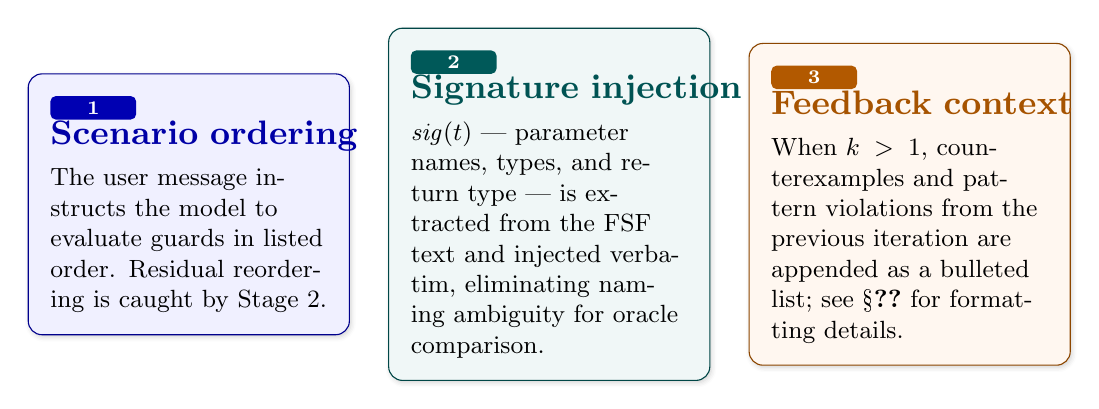
\begin{tikzpicture}[
  font=\small,
  card/.style={
    draw=#1!55!black, fill=#1!6, rounded corners=5pt,
    minimum width=0.31\linewidth, text width=0.29\linewidth,
    align=left, inner sep=8pt,
    blur shadow={shadow xshift=0.6pt, shadow yshift=-0.8pt,
                 shadow blur steps=4, shadow opacity=18}
  },
  tag/.style={
    font=\scriptsize\bfseries, text=white, fill=#1!70!black,
    rounded corners=2pt, inner sep=2pt
  }
]

\node[card=blue] (ord) at (0, 0) {%
  \tikz[baseline=(b.base)]{\node[tag=blue] (b) {1};}\hspace{0.35em}%
  \cardtitle{blue}{Scenario ordering}\\[4pt]
  The user message instructs the model to evaluate guards
  in listed order. Residual reordering is caught by Stage~2.};

\node[card=teal, right=0.04\linewidth of ord] (sig) {%
  \tikz[baseline=(b.base)]{\node[tag=teal] (b) {2};}\hspace{0.35em}%
  \cardtitle{teal}{Signature injection}\\[4pt]
  $\mathit{sig}(t)$ — parameter names, types, and return type —
  is extracted from the FSF text and injected verbatim,
  eliminating naming ambiguity for oracle comparison.};

\node[card=orange, right=0.04\linewidth of sig] (fb) {%
  \tikz[baseline=(b.base)]{\node[tag=orange] (b) {3};}\hspace{0.35em}%
  \cardtitle{orange}{Feedback context}\\[4pt]
  When $k > 1$, counterexamples and pattern violations from
  the previous iteration are appended as a bulleted list;
  see \S\ref{sec:method:repair} for formatting details.};

\end{tikzpicture}
